\subsubsection{Accounts and Business Access}
User is the application identity with a separate administrator/standard system role;
Worker is a business-specific person with no
required login. Workspace separates one owner's properties, campaigns and records.
WorkspaceMembership carries the contextual Owner/Manager role; each active
workspace has one Owner and an account owns at most one workspace.
ManagerInvitation records recipient and reviewed initial grants; acceptance requires
the intended verified account. AccessGrant records actual operations and scope,
including the mandatory insurance constraint. Revocation preserves author/initiator
references. Email verification challenges do not change the User id or ownership.
Workspace stores its business timezone. AccessGrant is keyed by membership,
operation and required property; scopes include parcels and current/future campaigns.
WorkerAvailability links explicitly available workers to manager membership before
scoped work exists; other relevant workers follow authorised scoped records.
It confers no other-property work visibility. Business closure and ownership
transfer are excluded. Account/data erasure requests require the separate privacy
procedure under \decisionref{Q-AA-07}; the model introduces no closure workflow.
Figure~\ref{fig:er-access} summarises the access relationships.

\begin{figure}[!htbp]\centering
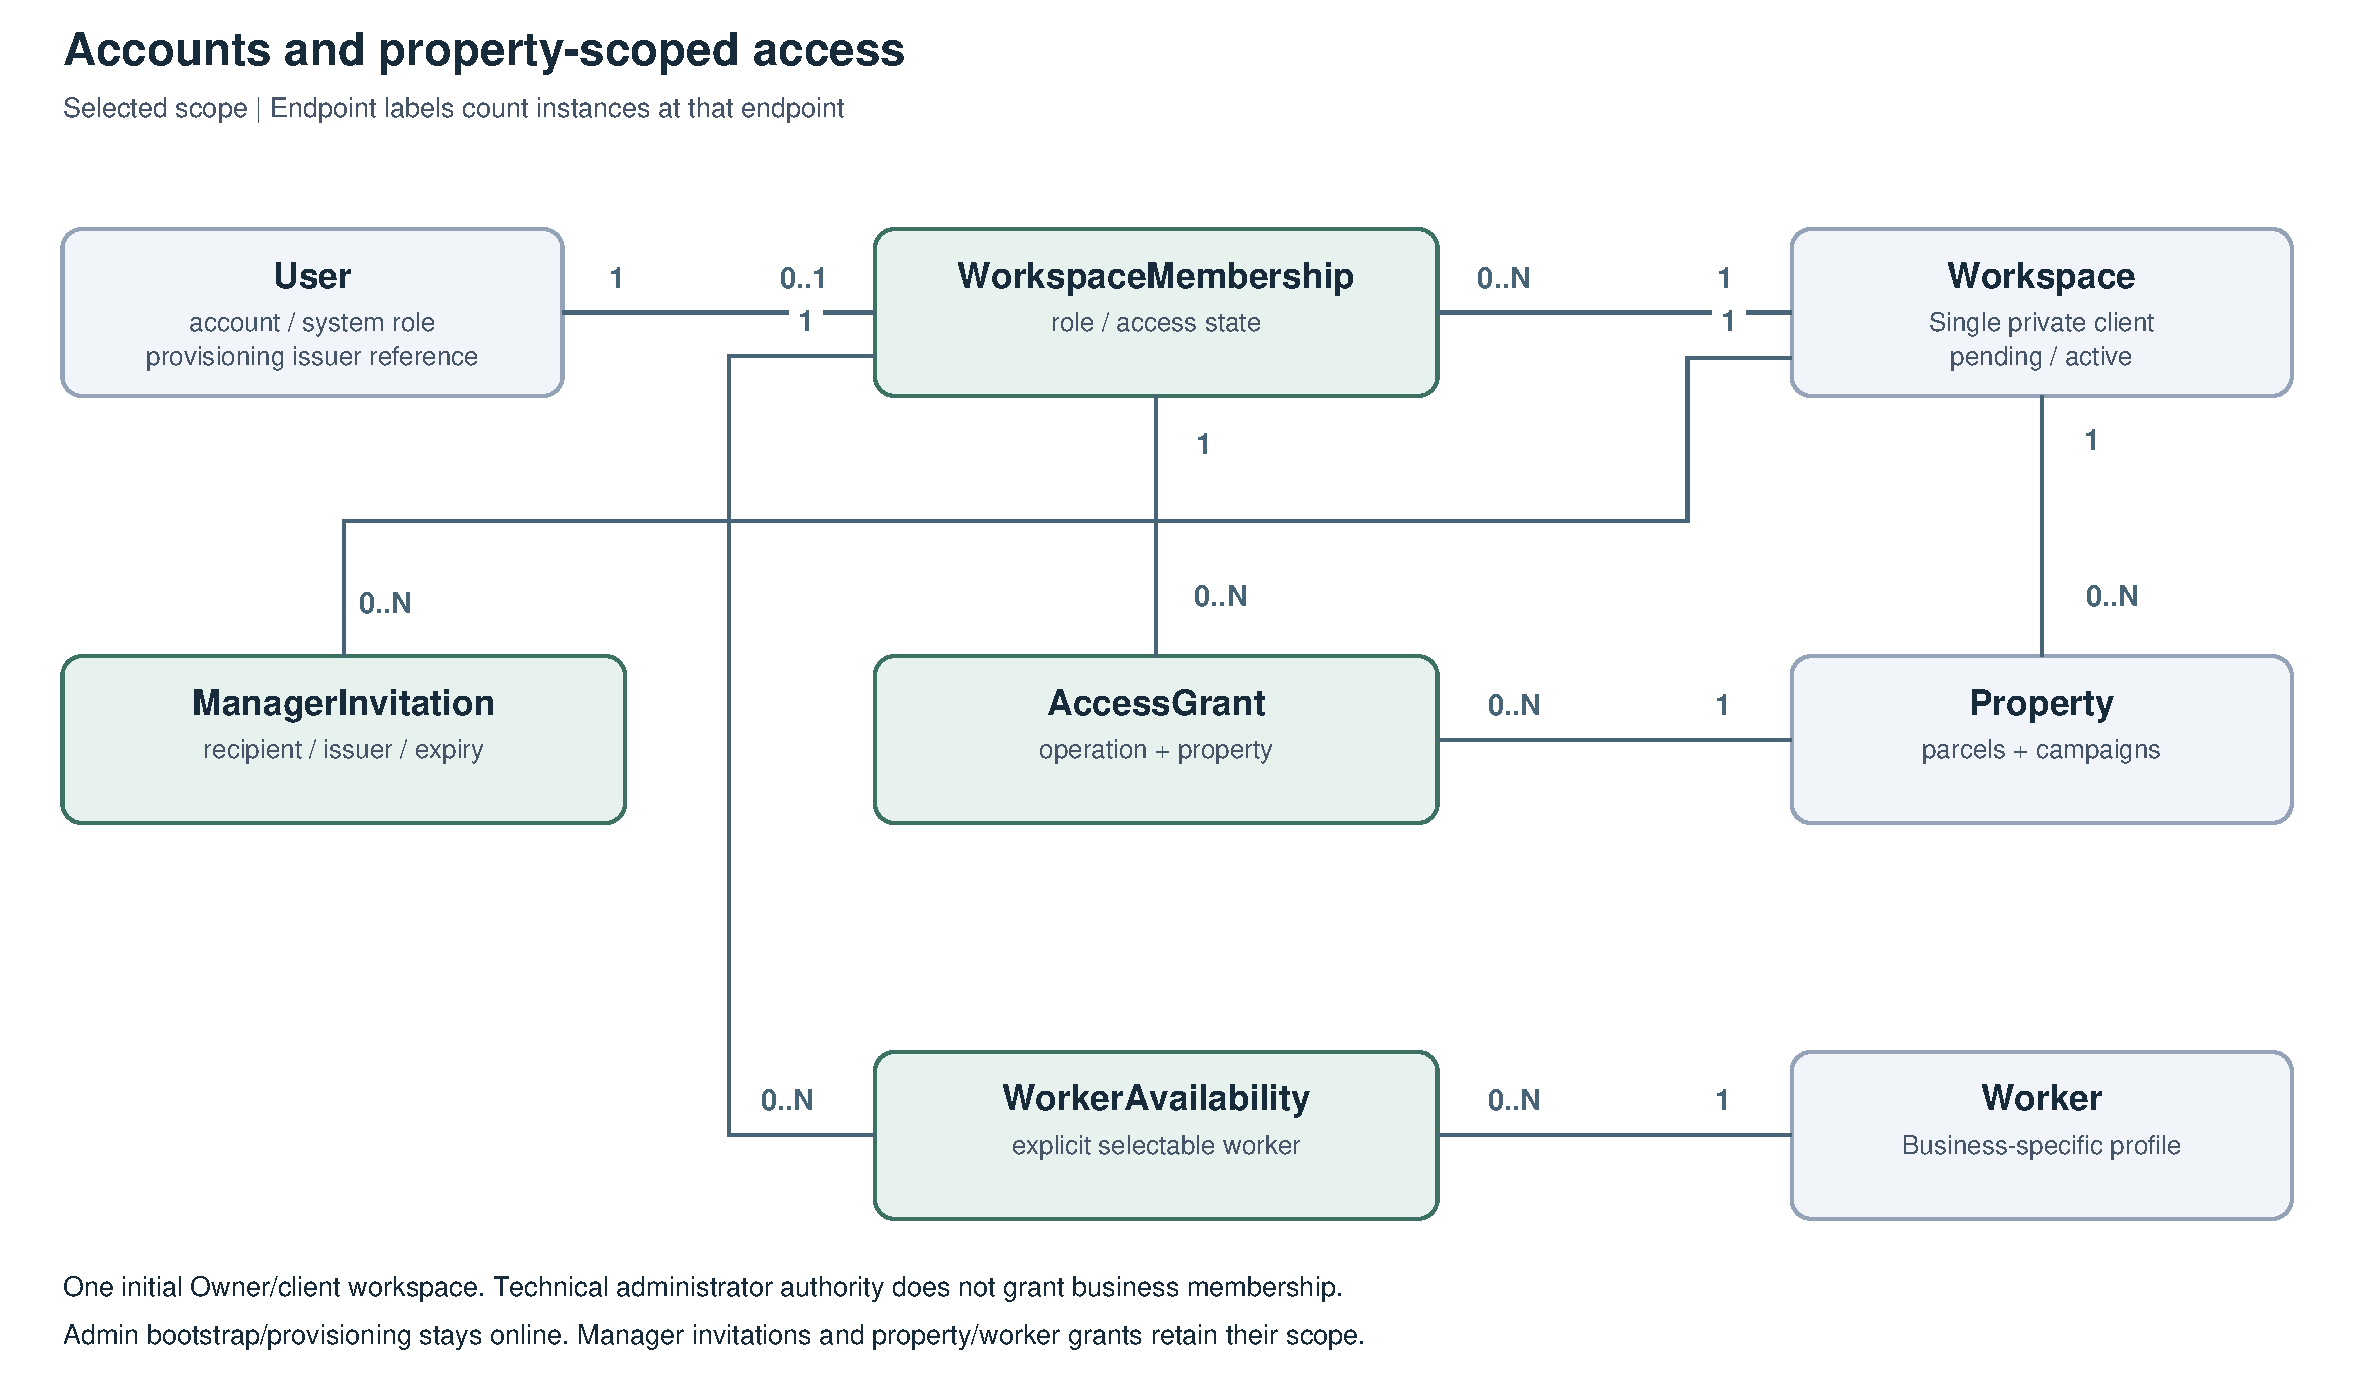
\includegraphics[width=\linewidth]{er-access.pdf}
\caption{Included account, membership, invitation and owner-configured access relationships.}
\label{fig:er-access}
\end{figure}

\paragraph{Provisioning.}
The administrator system role enables initial owner and workspace setup and activation
support only. Owner/Manager remain the operational membership roles. Bootstrap the
first administrator through deployment configuration, with no public administrator
signup. A nullable administrator reference on the provisioned owner records who
initiated setup. The owner workspace and membership remain pending until verified
activation; manager memberships still arise through accepted owner invitations.
The single-client deployment guard prevents a second initial owner/workspace.
